\section{Treinando o Stanford Parser sobre CINTIL}
\label{treinando_sp_cintil}

O pacote obtido, com o CINTIL, contém um guia de instruções (\cite{narrativeDescriptionCintil}), e o \textit{treebank} propriamente dito em formato XML\footnote{\url{https://www.w3.org/XML/}}. Para melhor uso, e melhor aplicação das árvores tanto para treino como para testes, fez-se necessária a separação deste arquivo em arquivos menores. Foi construído um \textit{script} na linguagem Python para fazer tal separação, gerando dois tipos de arquivo: as sentenças originais (\textquote{\textit{raw}}), e suas árvores (\textquote{\textit{tree}}).

Este único trabalho não é suficiente. As \textit{POS tags} do CINTIL estão em Português, e para o uso delas pelo SP sem uso de pacotes, seria necessário traduzi-las para o Inglês. Fizemos então a conversão dessas \textit{tags}, de acordo com a Tabela \ref{tab:tab_cintil}. Note que \textit{tags} que possuem tradução direta (exemplo: Adjetivo, A e JJ) não foram especificadas nas observações.

Outra dificuldade é que, como supracitado, o \textit{tagset} informado no site oficial do CINTIL está defasado com relação ao \textit{treebank} real. O \textit{tagset} mais confiável, a respeito, é o \textquote{CINTIL TreeBank Handbook} \cite{cintil_handbook}. Foram usadas as \textit{tags} listadas nele, e as que ocorrem no \textit{treebank} concreto e que não foram previstas no \textit{Handbook} (Por exemplo, P’, C’ etc).

\begin{center}
\begin{longtable}{|p{0.15\linewidth}|p{0.2\linewidth}|p{0.15\linewidth}|p{0.15\linewidth}|p{0.3\linewidth}|}
\caption{Tabela de conversão: CINTIL para PTB}\\
\hline
\textbf{Tag Original (Português)} & \textbf{Nome da Tag} & \textbf{Tag Convertida} & \textbf{Ocorrências} & \textbf{Observações}\\
\hline
\endfirsthead
\multicolumn{5}{c}%
{\tablename\ \thetable\ -- \textit{Continuação da página anterior}} \\
\hline
\textbf{Tag Original (Português)} & \textbf{Nome da Tag} & \textbf{Tag Convertida} & \textbf{Ocorrências} & \textbf{Observações} \\
\hline
\endhead
\hline \multicolumn{5}{r}{\textit{Continua na próxima página}} \\
\endfoot
\hline
\endlastfoot
    A & Adjetivo & JJ & 5527 & \\
    A' & Sintagma Adjetival & ADJP & 114 & \\
    ADV & Advérbios & RB & 5510 & \\
    ADV' & Sintagma Adverbial & ADVP & 912 & \\
    ADVP & Sintagma Adverbial & ADVP & 428 & \\
    AP & Sintagma Adjetival & ADJP & 1456 & \\
    ART & Artigo & DT & 15583 & \\
    ART' & Artigo & NP & 1 & Equivaleria ao constituinte interemediário do \textit{Determiner Phrase} (DP) \citeonline{mioto2013novo}. Porém, PTB não prevê esse tipo de estrutura. O sintagma mais indicado para receber determinantes (artigos) foi, portanto, NP\\
    C & Complementador & CC & 275 & Será explicado na sessão \ref{subsec-cintil-c}\\
    C' & Sintagma Complemental & \_CP\_ & 2 & Será explicado na sessão \ref{subsec-cintil-c}\\
    CARD & Cardinais & CD & 2028 & Números cardinais\\
    CARD' & Sintagmas Cardinais & NP & 504 & PTB prevê que conjuntos de números são marcados como NP\\
    CL & Clíticos & PRP & 717 & No CINTIL, ocorre apenas como pronome. De acordo com \citeonline{cintil_handbook}, \textquote{\textit{A clitic pronoun has category CL. It is the head of an NP.}}\\
    CONJ & Conjunções & CC & 2460 & Será explicado na sessão \ref{subsec-cintil-conj}\\
    CONJ' & Sintagma Conjuntivo & \_CONJP\_ & 92 & Será explicado na sessão \ref{subsec-cintil-conj}\\
    CONJP & Sintagma Conjuntivo & CONJP & 609 & Será explicado na sessão \ref{subsec-cintil-conj}\\
    CP & Sintagma Complemental & SBAR & 1434 & Será explicado na sessão \ref{subsec-cintil-c}\\
    D & Artigo & DT & 29 & \\
    D1 & Quantificadores & DT & 1 & Não ocorre no Handbook, só no site. Único caso em que essa \textit{tag} aparece, D1 se comporta como Artigo\\
    D2 & Quantificadores & JJ & 1 & Não ocorre no Handbook, só no site. Único caso em que essa \textit{tag} aparece, D2 se comporta como Adjetivo\\
    DEM & Demonstrativos & DT & 1013 & Para o PTB, \textit{this}, \textit{that}, \textit{these}, \textit{those} são, também, determinantes. Logo, DT\\
    ITJ & Interjeições & UH & 4 & \\
    ITJ' & Sintagma de Interjeição & INTJ & 4 & Pelo manual de \textit{bracketing} do PTB, \textquote{\textit{INTJ | Interjection. Corresponds approximately to the part-of-speech tag UH (see the POS guidelines [Santorini 1990]).}}\footnote{\textquote{Interjeição. Corresponde aprocimadamente à etiqueta morfossintática UH (veja as diretrizes [\citeonline{posPTBguidelines}]}. Tradução própria.}\\
    N & Substantivo & NNS & 32989 & \\
    N' & Sintagmas Nominais & NP & 18043 & \\
    NP & Sintagmas Nominais & NP & 32258 & \\
    ORD & Ordinais & CD & 378 & PTB não prevê o uso de ordinais. Ou melhor: eles costumam ser postos em locuções nominais.\\% Não é uma boa transdução\\
    P & Preposição & IN & 13920 & \\
    P' & Sintagmas Preposicionais & PP & 337 & Não ocorre no Handbook\\
    PERCENT & simbolo percentual & NN & 164 & Nota 1: pode ser pronome + substantivo também (\textquote{por cento}). Nota 2: PTB considera o \% como NN (\textit{single noum})\\
    PERCENT' & Sintagma percentual & NP & 80 & PTB considera como NP\\
    PERCENTP & Sintagma percentual & NP & 36 & \\
    PNT & Pontuação & ? & 14748 & Explicado na sessão \ref{subsec:cintil-pnt}\\
    POSS & Possessivos & PP\$ & 620 & \\
    POSS' & Possessivos & NP & 10 & Não existe um sintagma pronominal no PTB. Mantivemos como NP\\
    PP & Sintagmas Preposicionais & PP & 15382 & \\
    PRS & Pronomes Pessoais & PRP & 395 & \\
    QNT & Quantificadores & PRP & 889 & De acordo com (\citeonline[p~55]{Castilho2010gramatica}), \textquote{Os pronomes abrigam as seguintes subclasses [...]: pessoais, demonstrativos, possessivos e quantificadores [...]}\\
    QNT' & Sintagma de Quantificadores & NP & 19 & Como supracitado, se refere ao sintagma que abriga quantificadores (pronomes)\\
    REL & Relativos & PRP & 861 & Pronomes relativos\\
    S & Sentença & S & 24393 & \\
    V & Verbos  & VB & 13281 & \\
    V' & Sintagma Verbal & VP & 2745 &  \\
    VP & Sintagma Verbal & VP & 15284 & 
\label{tab:tab_cintil}
\end{longtable}
\end{center}

Como veremos também ao trabalharmos com o Bosque, nem todo caso pode ser feito com uma simples tradução direta CINTIL $\rightarrow$ PTB. Em alguns momentos, tivemos que avaliar, para cada caso, como traduzir a \textit{tag} de maneira correta. Estes casos serão descritos abaixo
% ------------------------------------------------------------------------------------------------
\subsection{Problemas com CONJ (Conjunção)}
\label{subsec-cintil-conj}
Conjunções são estruturas (palavras, no geral) que fazem parte da categoria semântica da Conectividade. Descrita por \citeonline[p~133]{Castilho2010gramatica},
\begin{displayquote}
    \textquote{Outra categoria semântica é a conectividade, gramaticalizada como preposições e conjunções. Essas classes ligam palavras e sentenças, com a diferença de que as preposições, como classe igualmente predicadora, atribui ao seu escopo traços de lugar, tempo, entre outros, propriedade não exercida pelas conjunções.}
\end{displayquote}
O mesmo autor descreve que sentenças podem ser ligadas por conjunções e que, ao fazê-lo, estamos criando uma relação conjuncional entre ambas. \citeonline[p~338]{Castilho2010gramatica}:
\begin{displayquote}
    \textquote{Essa relação compreende a [\ldots] coordenação, [\ldots] formada por sentenças independentes umas de outras, ou de [\ldots] subordinação, [\ldots] formada por sentenças encaixadas umas em outras, tanto quanto [\ldots] formada por uma sentença adjunta à outra.}
\end{displayquote}
A Tabela 
% \ref{tab:tab_conj_separadas_cintil} e 
\ref{tab:tab_conj_concat_cintil} mostra palavras e expressões utilizadas pelo CINTIL como conjunções.
% \begin{center}
% \begin{table}[!ht]
    \centering
    \begin{tabular}{|l|l|l|l|}
        \hline
        a & e & nem & se\\
        ainda & em & não & sem\\
        assim & em\_ & o & sempre\\
        até & embora & ou & só\\
        bem & enquanto & para & também\\
        caso & já & porque & tanto\\
        como & mais & quando & uma\\
        dado & mas & quanto & vez\\
        de\_ & medida & que & \\
        desde & mesmo & quer & \\
        \hline
    \end{tabular}
    \caption{Palavras únicas usadas como conjunções pelo cintil. Note que palavras com underline (\_) são concatenadas a outras (no geral, indica uma preposição)}
    \label{tab:tab_conj_separadas_cintil}
\end{table}
% \end{center}
\begin{center}
\begin{table}[!ht]
    \centering
    \begin{tabular}{|l|l|}
        \hline
        ainda que&mas\\
        até que&mesmo que\\
        dado que&ou\\
        de\_ o que&para que\\
        desde que&sem que\\
        e&tanto mais que\\
        em\_ a medida em que&uma vez que\\
        já que&\\
        \hline
    \end{tabular}
    \caption[Expressões usadas como conjunções pelo CINTIL]{Expressões (conjuntos de palavras, ou palavras únicas) usadas como conjunções pelo CINTIL. Note que as preposições com \textit{underline} se concatenam ao artigo posterior (de\_ + o = do)}
    \label{tab:tab_conj_concat_cintil}
\end{table}
\end{center}
O \textit{Penn Treebank} e o CINTIL lidam com conjunções de maneiras distintas. O PTB, em seu manual de anotação (\cite[p~117]{bracketing_ptb}), dedica a seção 7.5 para descrever tal fenômeno. Lá podemos ver que, para conjunções coordenadas, temos três casos: palavra simples (\textit{and}, \textit{but}, \textit{or}, \ldots), multi palavra (\textit{as well as}, \textit{not to mention}, \textit{rather than}, \ldots), e conjunções descontínuas (\textit{not only\ldots but}, \textit{not\ldots but instead}, \ldots). Palavras simples não precisam de marcação, a conjunção fica sem rótulo, como na Figura \ref{fig:ptb_conj_exe_1}. Conjunções com várias palavras tem o sintagma de conjunção marcado como CONJP, e as conjunções são postas em estrutura plana, mostrado na Figura \ref{fig:ptb_conj_exe_2}. Por fim, conjunções descontínuas tem apenas a parte com múltiplas palavras marcada por CONJP. A palavra isolada permanece isolada e sem marcação, como na Figura \ref{fig:ptb_conj_exe_3}. O manual possui a descrição de mais casos, envolvendo Conjunções Coordenadas e \textit{times}\footnote{\textit{Vezes}, no sentido de multiplicação. Exemplo, \textit{three times}, ou \textit{three times five}}, porém não nos alongaremos no assunto, por não possuírem as \textit{tags} CONJ ou CONJP.
\begin{center}
\begin{figure}[!h]
    \centering
    % \includegraphics{}
    \begin{minipage}{10cm}
        \begin{tabbing}
            \=(NP \=(NP a hammer)\+\\
            \>\textbf{and}\\
            \>(NP a nail))\\
        \end{tabbing}
    \end{minipage}
    \caption[Exemplo de conjunção coordenada (\textit{single-word})]{Exemplo de conjunção coordenada com uma palavra (\textit{single-word}). Adaptado de \citeonline[p~130]{bracketing_ptb}}
    \label{fig:ptb_conj_exe_1}
\end{figure}
\end{center}
\begin{center}
\begin{figure}[!h]
    \centering
    % \includegraphics{}
    \begin{minipage}{10cm}
        \begin{tabbing}
            \=(S (\=NP-SBJ That)\+\\
                \>(VP \=builds\+\\
                    \>(NP (NP confidence)\\
                    \>,\\
                    \>(NP self sufficiency)\\
                    \>,\\
                    \>\textbf{(CONJP not to mention)}\\
                    \>(NP critical regulatory net worth)))\-\\
                \>.)
        \end{tabbing}
    \end{minipage}
    \caption[Exemplo de conjunção coordenada \textit{multi-word}]{Exemplo de conjunção coordenada com muitas palavras (\textit{multi-word}). Adaptado de \citeonline[p~131]{bracketing_ptb}}
    \label{fig:ptb_conj_exe_2}
\end{figure}
\end{center}
\begin{center}
\begin{figure}[!h]
    \centering
    % \includegraphics{}
    \begin{minipage}{10cm}
        \begin{tabbing}
            \=(S (\=NP-SBJ The proposal)\+\\
                \>(VP \=represents\+\\
                    \>(NP \=\textbf{(CONJP not alone)}\+\\
                    \>(NP his own district)\\
                    \>\textbf{but}\\
                    \>(NP (NP all the people)\\
                    \>(PP \=of\\
                        \>(NP our country))))))\\
        \end{tabbing}
    \end{minipage}
    \caption[Exemplo de conjunção discontínua]{Exemplo de conjunção discontínua (\textit{discontinuous conjunction}). Adaptado de \citeonline[p~131]{bracketing_ptb}}
    \label{fig:ptb_conj_exe_3}
\end{figure}
\end{center}
O CINTIL, por outro lado, não é tão descritivo. É dito em \cite[p~20]{cintil_handbook}:
\textquote{\textit{Coordination of two constituents A and B by means of a coordinative conjunction Conj (either a lexical item, such as \textit{e}, or a comma) are a cascade of adjunctions [A [Conj [ B ]]].}}
\footnote{\textquote{Coordenação de dois constituintes A e B no sentido de uma conjunção coordenada Conj (tanto um item lexical, como \textit{e}, ou uma vírgula) são uma cascata de adjunções [A [Conj [B]]].}}
% Ele prevê as tags CONJ, CONJP e CONJ’.
Pela observação do \textit{treebank}, vemos CONJP se refere a toda a nova sentença em conjunção com a sentença inicial. CONJ’ se refere ao núcleo da conjunção (aos moldes da estrutura CP, que pode ser vista em \cite[p~63]{mioto2013novo}). Por fim, CONJ é a \textit{POS tag} referente a conjunções.

CINTIL abarca toda a nova sentença da conjunção, como demonstrado na Figura \ref{fig:cintil_conj_exe_1}. Como visto anteriormente, o mesmo não ocorre no PTB. Conjunções normalmente não são marcadas e, se forem, receberam a marca CONJP para o núcleo.
% \footnote{Também ocorre a conjunção marcada por SBAR, mas não há necessidade de explorarmos. Para o leitor curioso, recomendamos a leitura de \citeonline[sec~1.2.3]{bracketing_ptb}}1.
\begin{center}
\begin{figure}[!h]
    \centering
    % \includegraphics{}
    \begin{minipage}{.8\textwidth}
        \begin{tabbing}
            \=(S  \=\+\\
            \>    (S  \=\+\\
            \>        (NP  \=\+\\
            \>            (ART o) (N Manuel)\-\\
            \>        )\\ 
            \>        (VP  \=\+\\
            \>            (V é\=) \\
            \>            (AP \+\\
            \>               (A maior) \\
            \>                (CON\=JP \+\\
            \>                    (CON\=J' \+\\
            \>                        (CONJ de\_) (CONJ o) (CONJ que)\-\\
            \>                    ) \\
            \>                    (NP \=\+\\
            \>                        (ART A) (N Maria)\-\\
            \>                    ))))) \-\-\-\-\\
            \>    (PNT .)\-\\
            \>)
        \end{tabbing}
    \end{minipage}
    \caption[Exemplo de conjunção no CINTIL]{Sentença aTSTS-001/36, \textquote{o Manuel é maior do que A Maria}. Exemplo de conjunção no CINTIL (Adaptado)}
    \label{fig:cintil_conj_exe_1}
\end{figure}
\end{center}
Com isto em mente, fez-se necessário reescrever a disposição das \textit{tags}, para que: CONJP se referisse apenas aos núcleos conjuntivos, CONJ’ fosse removida e, no contexto em que CONJ aparece dentro de \textit{tags} CONJP, remover suas marcações, sem removê-las noutros momentos. Um exemplo pode ser visto na Figura \ref{fig:cintil_conj_exe_2}.
\begin{center}
\begin{figure}[!ht]
    \centering
    % \includegraphics{}
    \begin{minipage}{10cm}
        \begin{tabbing}
            \=(S\=\+\\ 
            \>  (S\=\+\\ 
            \>    (NP\=\+\\ 
            \>      (DT o)\\
            \>      (NNS Manuel)\=\-\-\\
            \>    )\\
            \>    (VP\=\+\\ 
            \>      (VB é)\\
            \>      (ADJP\=\+\\ 
            \>        (JJ maior)\\
            \>        (CONJP de\_ o que)\\
            \>        (NP\=\+\\ 
            \>          (DT A)\\
            \>          (NNS Maria)\-\\
            \>        )\-\\
            \>      )\-\\
            \>    )\-\\
            \>  )\\
            \>  .)\\
        \end{tabbing}
    \end{minipage}
    \caption[Sentença aTSTS-001/36, modificada para se adaptar ao PTB]{Sentença aTSTS-001/36, \textquote{o Manuel é maior do que A Maria.}, modificada pelo algoritmo desenvolvido para se adaptar ao PTB}
    \label{fig:cintil_conj_exe_2}
\end{figure}
\end{center}

\subsection{Problemas com C (Complementizador)}
\label{subsec-cintil-c}
Semelhante à CONJ em diversos aspectos, as \textit{tags} C, C’ e CP permitem a conjunção entre sentenças, tornando uma segunda sentença objeto de uma primeira. O tratamento feito com elas foi muito semelhante ao dado para a \textit{tags} CONJ, com um diferencial: CONJ’ ocorre sem necessariamente ter a \textit{tags} CONJP como pai (12 casos), o que nunca ocorre com a família CP. 

\subsection{Problemas com PNT (Pontuação)}
\label{subsec:cintil-pnt}
Foi observado, também, que CINTIL e PTB lidam com pontuações de formas distintas. CINTIL usa a \textit{tags} PNT para classificar estes símbolos. PTB prevê uma \textit{tags} SYM, para símbolos. Além disso, vemos em \cite[p~52]{buildingPTB} que os símbolos costumam ser representados sem etiquetas, como exemplificado na Figura \ref{fig:ptb_comma_parenthe}. Em \cite[p~52]{bracketing_ptb}, fica bastante claro: fora \textit{bracketing} (parênteses, colchetes, chaves), os símbolos não recebem nenhuma \textit{POS}. Quando recebe, como no caso de símbolos funcionando como palavras, ou símbolos matemáticos, são \textit{tags} referentes ao sintagma. Um detalhe importante é como PTB lida com aspas e apóstrofos (\textit{quote}, e \textit{single-quote}). As aspas são removidas, e substituídas por dois apóstrofos ou duas crases (melhor visualizado na Figura \ref{fig:ptb-quote}).

\begin{center}
    \begin{figure}[!ht]
    \centering
    % \includegraphics{}
    \begin{minipage}{10cm}
        \begin{tabbing}
            \=(   (S-1 \=\+\\ 
            \>    (PP-TMP \=For\+\\
            \>		(NP \=(NP the rest)\+\\
            \>			(PP \=of\+\\
            \>				\=(NP 1989))))\-\-\-\-\\
        	\>  (PRN \=,\+\\
            \>		(S \=(NP-SBJ Mr. Hagen) \+\\
            \>	        (VP \=said\+\\
            \>		        (SBAR \=0\+\\
            \>				    (S *T*-1))))\-\-\-\\
            \>		,)\-\\
            \>	(NP-SBJ \=(NP Conrail 's)\+\\
            \>		traffic and revenue)\-\\
            \>	''\\
            \>	(VP \=will\+\\
            \>		(VP \=reflect\+\\
            \>			(NP the sluggish economy)))\-\\
            \>	.))
        \end{tabbing}
    \end{minipage}
    \caption[Vírgulas marcando S entre parênteses]{Vírgulas marcando S entre parênteses (adaptado de \citeonline[p~52]{bracketing_ptb})}
    \label{fig:ptb_comma_parenthe}
\end{figure}
\end{center}

\begin{center}
    \begin{figure}[!h]
    \centering
    % \includegraphics{}
    \begin{minipage}{.8\textwidth}
        \begin{tabbing}
        \=((SINV \=\lq\lq\+\\
        \>    (S-TPC-1    \=(NP-SBJ We)\\
        \>                (VP \=have\+\\
        \>		            (NP \=(NP no useful information)\+\\
        \>			            (PP \=on\+\\
        \>			                (SBAR \=whether\+\\
        \>            				   (S \=(NP-SBJ users)\\
        \>            				      (VP \=are\+\\
        \>                					  (PP-\=PRD at\+\\
        \>                						  (NP risk)))))))))\\
        \>	\=, \\
        \>	\lq\lq\\
        \>  (VP \=said\+\\
        \>	    (S *T*-1))\-\\
        \>	(NP-\=SBJ (NP James A. Talcott)\+\\
        \>		(PP \=of\+\\
        \>		    (NP \=(NP Boston \lq s)\+\\
        \>			    Dana-Farber Cancer Institute)))\-\-\-\\
        \>	.))
        \end{tabbing}
    \end{minipage}
    \caption[Exemplo de uso de aspas no PTB]{Exemplo de uso de aspas no PTB (fragmento adaptado da sentença wsj\_0003)}
    \label{fig:ptb-quote}
\end{figure}
\end{center}

Fez-se necessário criar um \textit{script} que removesse as \textit{tags} PNT dos símbolos, do CINTIL, para reposicioná-los corretamente nas árvores, além de tratar \textit{quotes}.

% Porém, não podia ser tão simples, e não foi. 
Porém,
CINTIL não só identifica os PNT de forma diferentes, como também os POSICIONA de forma distinta, como podemos ver no comparativo da Figura \ref{fig:comp_PNT_ptb_cintil}. No exemplo, abordando ponto final, é definido em  \cite[p~52]{bracketing_ptb}, 
\begin{quote}
    \textquote{\textit{In this corpus, each unit of text is enclosed in a top level of unlabeled brackets [\ldots]. Formerly, top-level punctuation [\ldots] could be attached to these top-level brackets. However, in this release, such punctuation should all be attached one level down (to the highest level of labeled brackets), so that there is only one top-level node within the unlabeled brackets.}}
    \footnote{\textquote{Neste corpus, cada unidade de texto é fechada no nível superior de parênteses não marcados [\ldots]. Anteriormente, pontuações de nível superior [\ldots] podiam ser anexadas àqueles parênteses de nível superior. Porém, nesta versão, tal pontuação deve toda ser anexada um nível abaixo (para o nível mais alto dos parênteses rotulados), então existe apenas um nó no topo dentro dos parênteses não rotulados}. Tradução própria.}
\end{quote}
E resume em \citeonline[p~57]{bracketing_ptb}: 
\textquote{\textit{Final punctuation as a rule is a child of the highest level of structure}}.
\footnote{\textquote{Ponto final é, por regra, um filho da estrutura de nível mais elevado}. Tradução própria.}
Já \citeonline[p~29]{cintil_handbook} define como \textquote{\textit{End of sentence markers are in the top most adjunction}}
\footnote{\textit{Marcadores de fim de sentença estão na adjunção mais ao topo}. Tradução própria.}.

\begin{center}
    \begin{figure}[!h]
    \centering
    % \includegraphics{}
    \begin{minipage}{0.5\textwidth}
        \centering
        \begin{forest}
            [ [S [NP-SBJ This]
            [VP is
            [NP-RPD [NP John]
            [\textbf{,}]
            [NP my brother]]]
            [\textbf{.}]]]
        \end{forest}
        \caption{\textquote{This is John, my brother.}}
    \end{minipage}%
    % \hfill
    \begin{minipage}{0.5\textwidth}
        \centering
        \begin{forest}
            [S [S [VP [VP [ADV Assim]] [ADV' [\textbf{PNT ,}] [ADV' [ADV tal] [ADV e] [ADV qual]]]]] [\textbf{PNT .}]]
        \end{forest}
        \caption{\textquote{Assim, tal e qual.}}
    \end{minipage}
    \caption[Comparativo entre posicionamento de sinais de pontuação entre o Penn Treebank e o CINTIL]{Comparativo entre posicionamento de sinais de pontuação entre o Penn Treebank e o CINTIL.}
    \label{fig:comp_PNT_ptb_cintil}
\end{figure}


\end{center}

Vírgulas também são bastante curiosas. Em \cite[p~52]{bracketing_ptb}: 
\begin{quote}
    \textquote{\textit{Paired punctuation marks are siblings of the constituents they surround. This is true even when the opening or closing member of the pair can be viewed as deleted. For instance, the commas that set off a subordinate clause or a relative clause from a main clause are siblings of the SBAR dominating the subordinate clause. [\ldots]}}
    \footnote{\textquote{Marcadores de pontuação pareados são irmãos do constituinte que eles rodeiam. Isto é verdade mesmo quando o membro inicial ou final do par pode ser visto como apagado. Por exemplo, as virgulas que definem uma cláusula subordinada ou clausula relativa de uma cláusula principal são irmãos do SBAR dominando a cláusula subordinada. [\ldots]}. Tradução própria.}
\end{quote}
Podemos ver esse fenômeno na Figura \ref{fig:ptb_comma_parenthe}. Já em \cite[p~30]{cintil_handbook}, 
\textquote{\textit{Commas separating left periphery constituents are right adjoined to theses constituents.}}
\footnote{\textquote{Vírgulas separando constituintes periféricos à esquerda são adjungidos à direita destes constituintes}, tradução própria}, exemplo na Figura \ref{fig:cintil_comma_left}.

\begin{center}
    \begin{figure}[!h]
    \centering
    % \includegraphics{}
    \begin{forest}
		[S [PNT '] [S [S [VP [V Falámos] [PP [PP [P de] [NP [N caça]]] [PP [\textbf{PNT ,}] [PP [PP [P de\_] [NP [ART os] [N sócios]]] [PP [CONJ e] [PP [P de] [NP [N' [N assuntos] [PP [P de] [NP [N homens]]]]]]]]]]]] [PNT .]]]
    \end{forest}
    \caption[Exemplo de comportamento da vírgula no CINTIL]{Exemplo de comportamento da vírgula no CINTIL. Vírgulas separando componentes periféricos à esquerda são anexados à direita do constituinte. Adaptado de \citeonline[p~30]{cintil_handbook}}
    \label{fig:cintil_comma_left}
\end{figure}
\end{center}

Para o leitor curioso, fica o Capítulo 3 de \cite{bracketing_ptb}, e 12 de \cite{cintil_handbook}, para o estudo dos demais sinais.

Antes de encerrarmos, existem casos no \textit{treebank} em que pontuações não são associadas à etiqueta PNT. Esses casos costumam ser pontos de abreviação, reticências, ou apóstrofos (\textit{single-quotes}) que antecedem nomes, e estão associados à etiqueta N. Para resolvê-los, primeiro mudamos suas etiquetas para PNT. Depois, continuamos com as operações previstas.

Fica claro, então, que é necessário \textit{reposicionar} os sinais antes de passar as árvores processadas para o SP. 
% parece um erro pequeno, mas 
Tal erro inviabiliza completamente qualquer tipo de teste, como podemos ver na mensagem de retorno exibida na Figura \ref{fig:cintil_training_error}. Num primeiro momento, a solução foi apenas remover tais elementos, o que viabilizou o treinamento e avaliação.

\begin{center}
    \begin{figure}[!h]
    \centering
    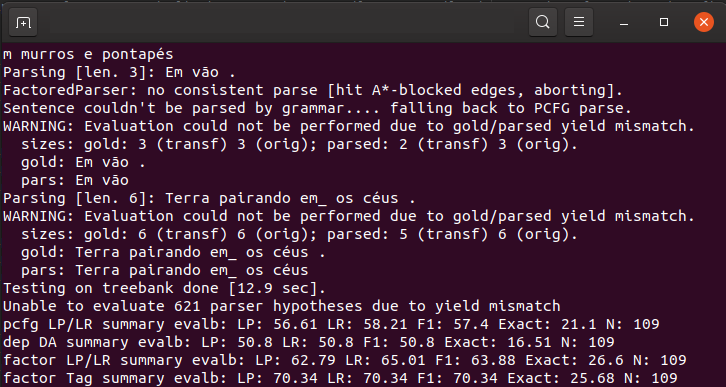
\includegraphics[width=100mm,scale=1.5]{imagens/cintil_training_error.png}
    \caption[Erro decorrente do mal posicionamento de pontuações na árvore do CINTIL]{Captura de tela de erro decorrente do mal posicionamento de pontuações na árvore do CINTIL, com relação ao formato PTB}
    \label{fig:cintil_training_error}
\end{figure}
\end{center}

% ------------------------------------------------------------------------------------------------
\subsection{Treinamento}\label{subsec:treinamento_cintil}
Para fazer estas conversões, fizemos um \textit{script} disponível online\footnote{\url{ https://github.com/Fernandomn/separador-cintil}}.

Com as \textit{tags} convertidas, foi feito o treinamento. O ato do treino é relativamente simples: deve-se, através do terminal do seu sistema, navegar até o diretório onde se encontra o \textit{stanford-parser.jar}, o arquivo que contém os \textit{parsers} do SP que utilizaremos. Estando no diretório correto, deve-se executar o comando \ref{lst:testeBasicoCintil}:

\begin{center}
\begin{lstlisting}[breaklines, caption={Execução de treinos do Stanford Parser para o CINTIL},label={lst:treinoBasicoCintil},language=Bash]
    java -cp ~/<diretorio de trabalho>/stanford-parser.jar -mx4g edu.stanford.nlp.parser.lexparser.LexicalizedParser -train ~/<diretorio do treebank>/tree-trad 1-1014 -saveToSerializedFile ~/<diretorio de armazenamento>/serialGrammarCINTIL -saveToTextFile ~/<diretorio de armazenamento>/textGrammarCINTIL
\end{lstlisting}
\end{center}

O código acima merece algumas explicações a parte, para quem não está familiarizado ao uso do SP pelo terminal.

\begin{center}
\begin{table}[h!]
    \centering
    \begin{tabular}{p{0.8\textwidth}}
        \begin{itemize}
            \item [-cp] \textit{ClassPath}. Indica o diretório onde se encontra a classe principal a ser executada
            \item [-mx4g] Quantidade de memória usada. No caso, 4 GB.
            \item [LexicalizedParser] \textit{Parser} utilizado, dentre os disponibilizados
            \item [-train] Treino. Logo em seguida, um diretório e a lista de arquivos a serem usados para treinar
            \item [-saveToSerializedFile] Salva o resultado do treino num arquivo binário, cujo diretório está indicado na sequência
            \item [-saveToTextFile] Salva o resultado do treino num arquivo de texto, cujo diretório está indicado na sequência
        \end{itemize}
    \end{tabular}
    \caption[Comandos para um treino simples do \textit{Stanford Parser}]{Comandos para um treino simples do \textit{Stanford Parser}, utilizando o terminal.}
    \label{tab:tab_treino_basico_cintil}
\end{table}
\end{center}

A Tabela \ref{tab:tab_treino_basico_cintil} mostra um fragmento das possibilidades de comandos a serem usados pela interface do terminal do SP. Note que usamos apenas 1014 arquivos nesta demonstração, que é um fração de 10\% dos arquivos / árvores do CINTIL disponíveis.

Para melhor verificação dos resultados, utilizamos o método de \textit{10-fold cross-validation}. Este método, como explicado por \citeonline{james2013introduction},
\begin{displayquote}
    \textquote{\textit{[\ldots] involves randomly dividing the set of observations into k groups, or folds, of approximately equal size. The first fold is treated as a validation set, and the method is fit on the remaining k -- 1 folds}}
    \footnote{\textquote{Esta abordagem envolve dividir aleatoriamente o conjunto de observações em k grupos, ou dobras, de tamanhos aproximadamente iguais. O primeiro grupo é tratado como conjunto de validação, e o método se encaixa nos k -- 1 grupos restantes}. Tradução própria.}.
\end{displayquote}

No nosso caso, dividimos nosso \textit{corpora} em 10 partes de 1014 sentenças. Fizemos o treinamento com 1 parte, e o teste com a parte restante, alternando as partes escolhidas.  Os resultados serão apresentados na conclusão.

Na sequência, foi executado o treinamento com as partes restantes. De maneira análoga, no mesmo diretório, foi utilizado o comando \ref{lst:testeBasicoCintil}:

\begin{center}
\begin{lstlisting}[breaklines, caption={Execução de testes do Stanford Parser para o CINTIL},label={lst:testeBasicoCintil},language=Bash]
    java -cp stanford-parser.jar -mx4g edu.stanford.nlp.parser.lexparser.LexicalizedParser -loadFromSerializedFile /home/fernando/projeto-final-parsers/serialized-files/serialGrammarCINTIL1 input/sentencas_teste_cintil.txt

\end{lstlisting}
\end{center}
Que também merece explicações, na Tabela \ref{tab:tab_teste_basico_cintil}:
\begin{center}
\begin{table}[h!]
    \centering
    \begin{tabular}{p{0.8\textwidth}}
        \begin{itemize}
            \item [-cp] \textit{ClassPath}. Indica o diretório onde se encontra a classe principal a ser executada
            \item [-mx4g] Quantidade de memória usada. No caso, 4 GB.
            \item [LexicalizedParser] \textit{Parser} utilizado, dentre os disponibilizados
            \item [-writeOutputFiles ] Indica que os testes imprimirão arquivos de saída, a serem definidos
            \item [-outputFilesDirectory] Define o diretório onde os arquivos de saída serão escritos. 
            \item [-loadFromSerializedFile] Carrega a gramática serializada, gerada na execução de treinamento anterior
            \item [-testTreebank] Diretório onde se encontra o treebank a ser usado para teste. Os números no formato $a-b$ indicam o primeiro e o último arquivo, respectivamente. Números no formato $a-b,c-d$ indicam dois blocos de arquivos. Atente para não usar o mesmo bloco dos treinos, ou o parser passará por \textit{overfitting}, e terá resultados enviesados.
        \end{itemize}
    \end{tabular}
    \caption[Comandos para um teste simples do Stanford Parser]{Comandos para um teste simples do Stanford Parser, utilizando o terminal.}
    \label{tab:tab_teste_basico_cintil}
\end{table}
\end{center}
O resultado total dos testes resultou na extensa Tabela \ref{tab:cintil_result_full}, que pode ser vista nos apêndices. E os comentários dos resultados pode ser encontrado em \ref{resultados_cintil}.